\chapter{Detección de bloques comerciales}

\section{Red de insumo-producto internacional (1995-2022)}

%%%%%%%%%%%%%%%%%%%%%%%%%%%%%%%
% 4 Trade Types - Xing (2022) p. 33 : 
%Comercio interindustrial  I (País A sector i vende a país B sector j, i!=j)
% comercio intraindustrial (II) (País A sector i vende a país B sector i)
%Comercio de insumo producto industrial (IV) (País A sector i -> i)
% comercio de autoconsumo industrial (III) (País A sector i -> j)
%%%%%%%%%%%%%%%%%%%%%%%%%%%%%%%4


El comercio intermedio global puede clasificarse en cuatro tipos, de acuerdo a si el flujo comercial se realiza dentro del mismo país o no, y si el intercambio de bienes y servicios se produce entre diferentes sectores:
\begin{itemize}
	\item Tipo I, comercio interindustrial (internacional): Corresponde al comercio de bienes y servicios entre diferentes sectores de diferentes países.
	\item Tipo II, comercio intraindustrial (internacional): Se refiere al intercambio de productos dentro del mismo sector, pero de diferentes países. 
	\item Tipo III, insumo-producto nacional: Es el comercio vertical entre diferentes sectores de un mismo país.
	\item Tipo IV, autoconsumo industrial: Es el comercio horizontal de productos dentro de un mismo sector y país \parencite[p.~33]{Xing2022}.
\end{itemize} 

Los flujos de comercio internacional están representados por el comercio tipo I y II; mientras que los flujos comerciales nacionales equivalen a la suma de los tipos III y IV. En la figura \ref{Fig_Esquema_TiposComercio} se presenta un esquema de los tipos de comercio intermedio en una MRIOT de 3 países con 4 sectores económicos.

\begin{figure}[h]
	\centering
	
\includegraphics[width=1\linewidth]{Esquema_TiposComercio_2.png}
	\caption{Comercio intermedio global.}
	\label{Fig_Esquema_TiposComercio}
\end{figure}

La figura \ref{Fig_Comercio_InternoExterno} muestra el porcentaje que representa el comercio nacional e internacional, respecto al comercio intermedio global, durante el periodo de estudio. Aunque los flujos comerciales dentro de los países siguen teniendo la mayor proporción; durante el periodo de 1995 y 2008, el comercio internacional aumentó su participación de forma sostenida, pasando del 10.6\% al 15.1\%. Este periodo estuvo marcado por la creación de la Organización Mundial del Comercio (OMC) el 1° de enero de 1995, el ingreso de China a esta organización el 11 de diciembre de 2001 y la entrada en circulación (física) del Euro el 1° de enero de 2002. El aumento relativo del comercio intermedio internacional indica un fortalecimiento de la globalización y del entrelazamiento de la producción en el mundo. La crisis económica de 2008 fue el punto de inflexión de este proceso, que implicó una caída en el peso relativo del comercio internacional frente al nacional. Después de ese año, la proporciones entre el comercio nacional e internacional han pasado por ciclos, con periodos donde el comercio internacional gana terreno frente al nacional (2009-2012, 2016-2018 y 2020-2022); y periodos donde retrocede (2012-2016, 2018-2020).


\begin{figure}[H]
	\begin{subfigure}{\textwidth}
		\centering
		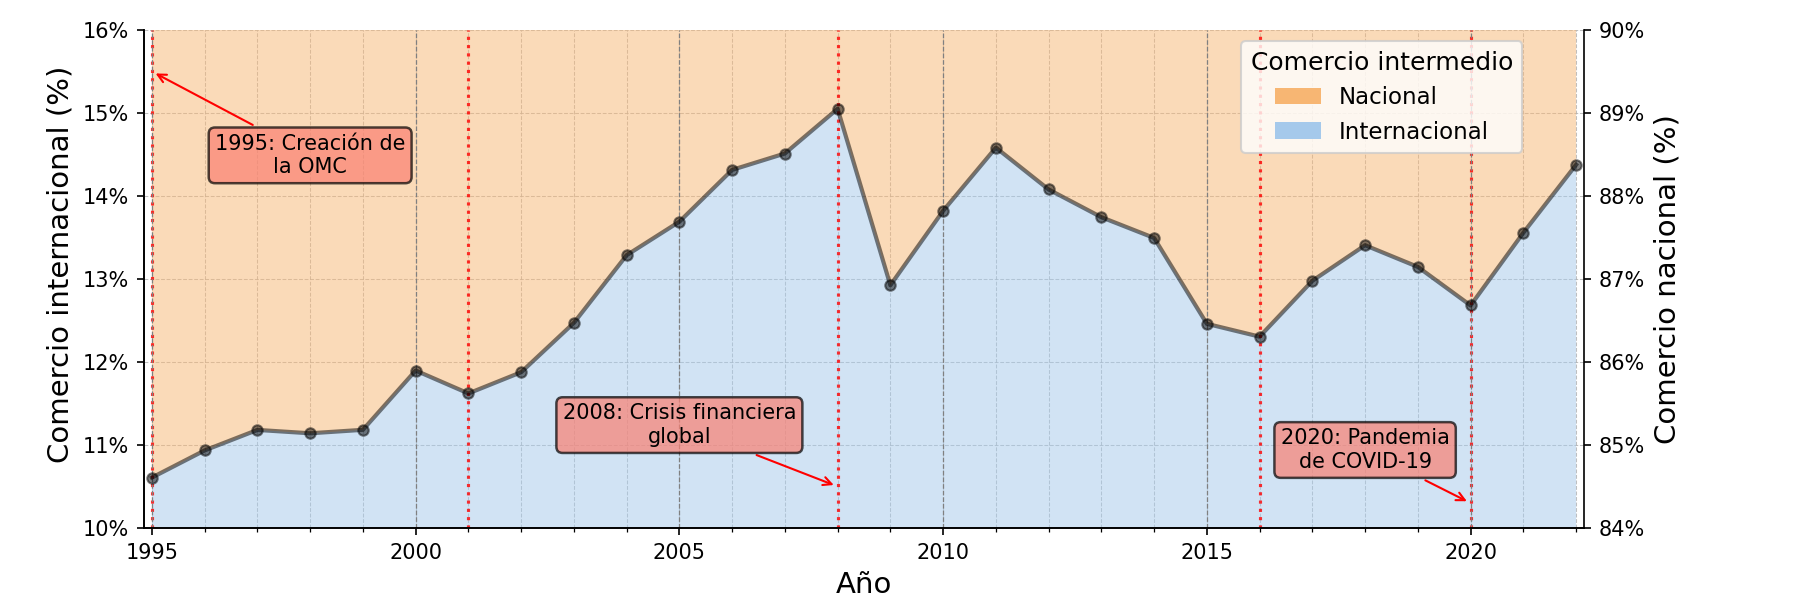
\includegraphics[width=\textwidth]{Comercio_InternoExterno.png}
		\caption{División nacional / internacional}
		\label{Fig_Comercio_InternoExterno}
	\end{subfigure}
	\begin{subfigure}{\textwidth}
		\centering
		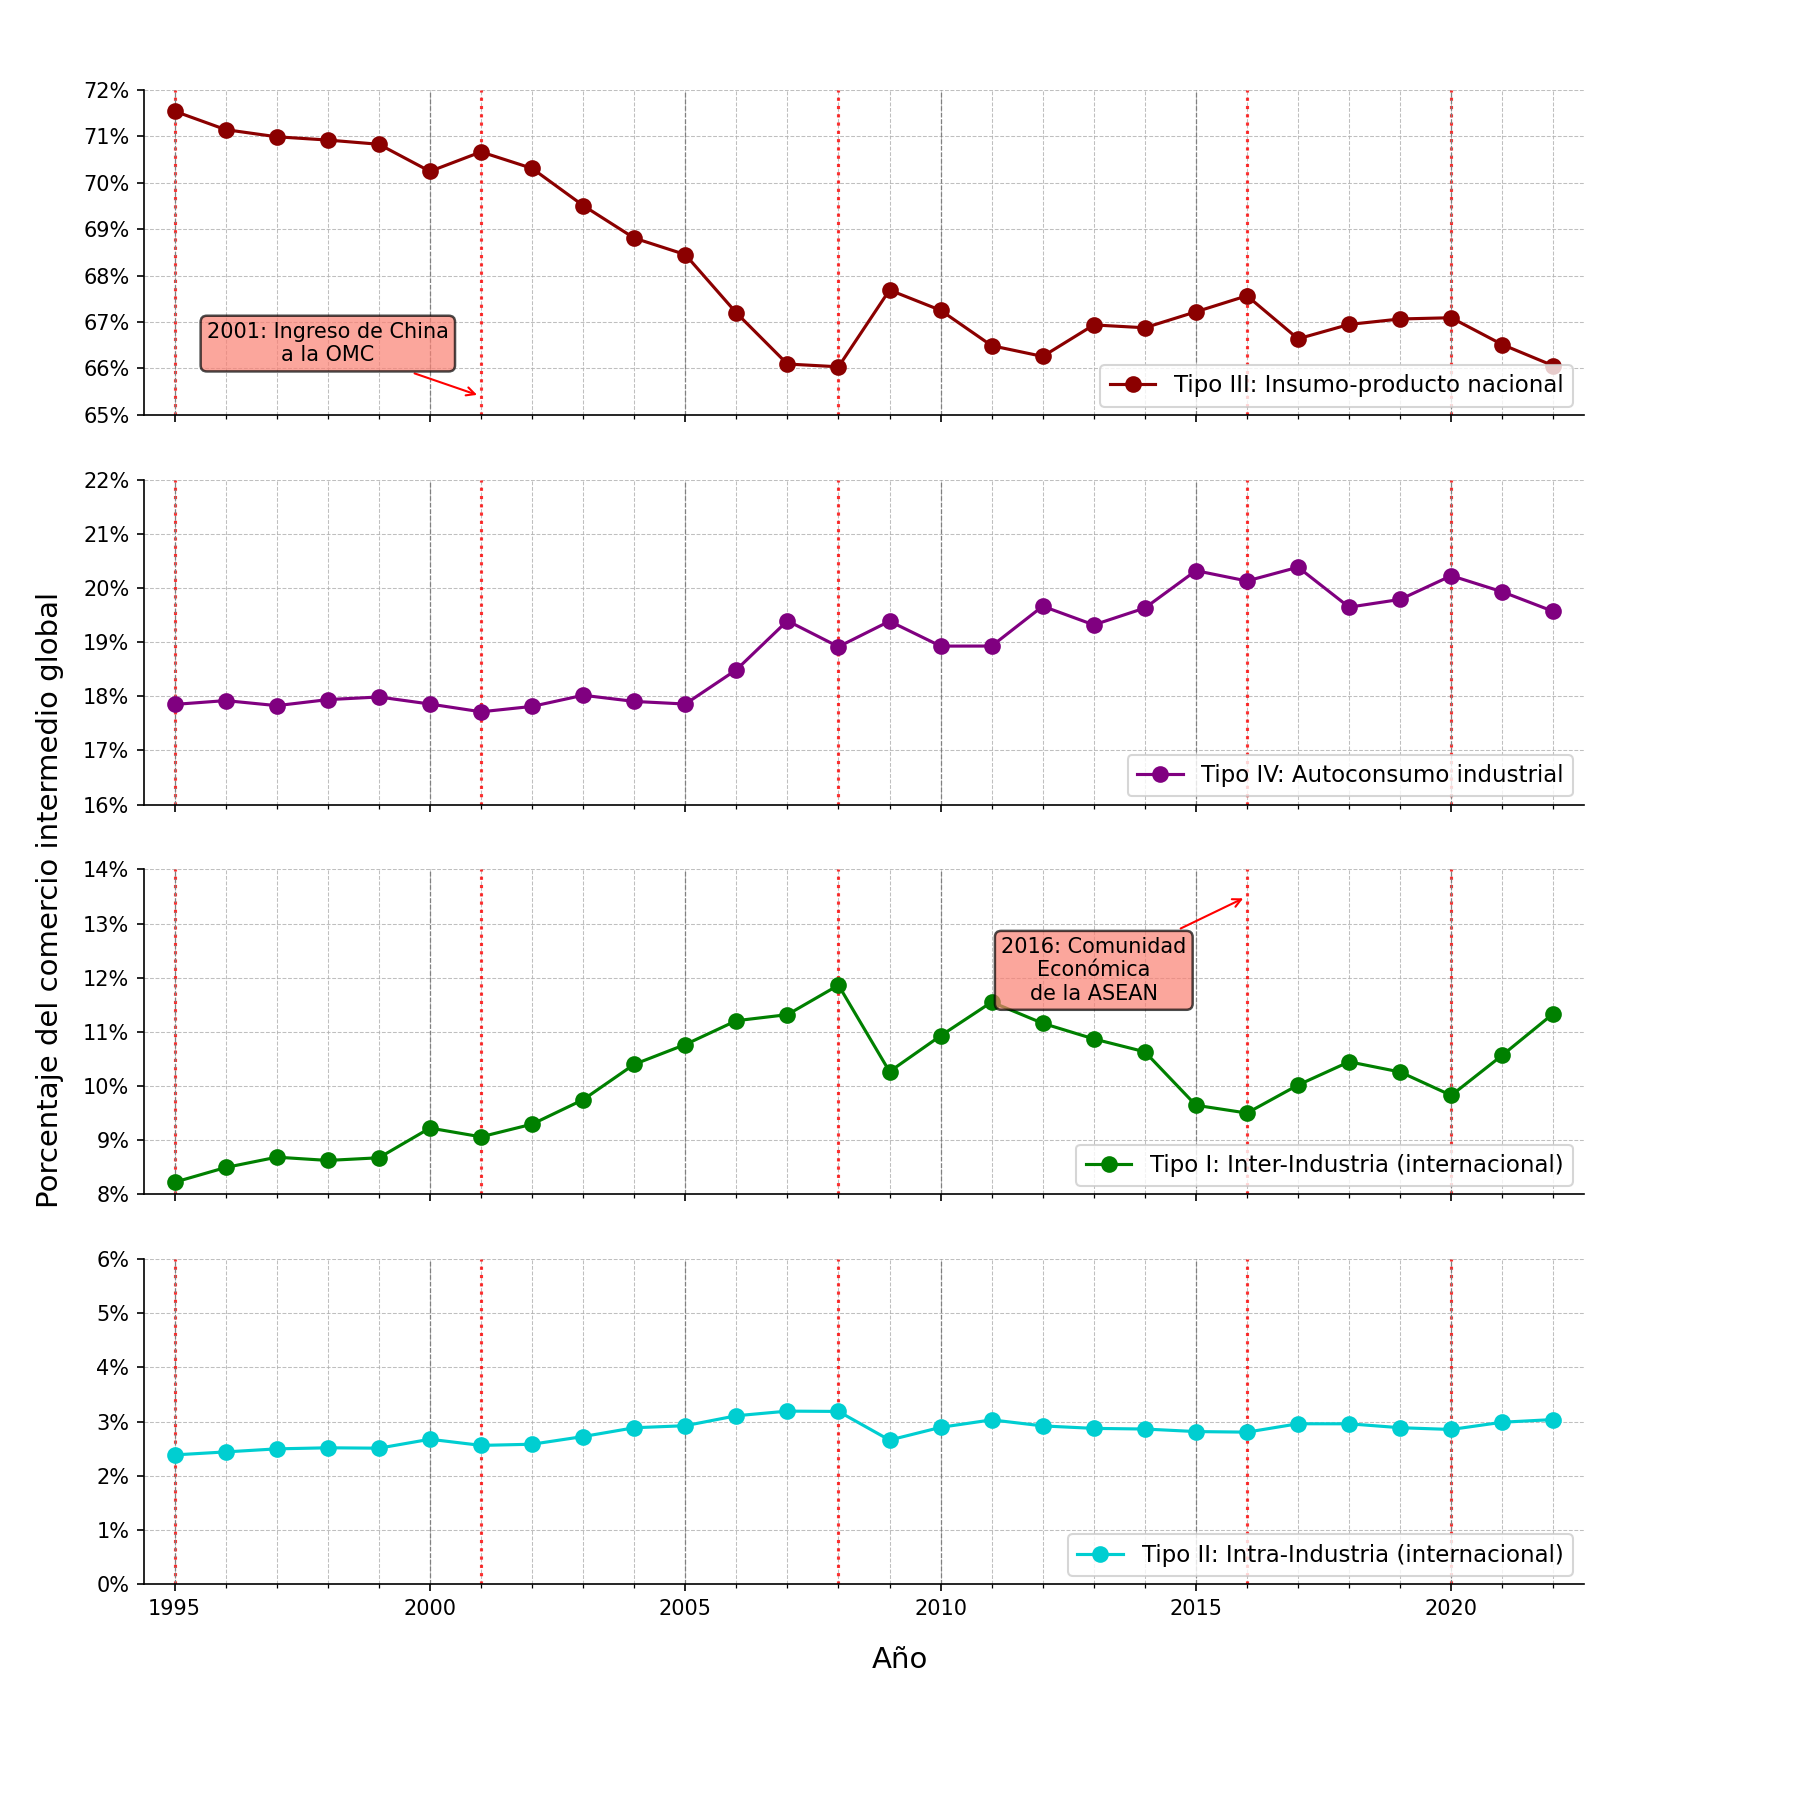
\includegraphics[width=\textwidth]{TipoComercio.png}
		\caption{Peso relativo por tipo de comercio}
		\label{Fig_TipoComercio}
	\end{subfigure}
	\caption{Evolución del comercio intermedio global}
\end{figure}

Una revisión más detallada de los datos sugiere que la crisis de 2008 no implicó un retroceso permanente en la globalización, pero si una reconfiguración de las cadenas globales de valor. En la figura \ref{Fig_TipoComercio} aparece el peso relativo de cada tipo de comercio intermedio. El primer bloque, correspondiente al porcentaje del comercio insumo-producto nacional, presenta una caída sostenida de 1995 ($71.5\%$) a 2008 ($66\%$); y posteriormente parece estabilizarse alrededor del $67\%$. Por otra parte, los pesos relativos del comercio de tipo I y IV ponen de manifiesto que la pérdida del peso relativo en el comercio interindustrial internacional a partir de 2018 fue ocupada por el crecimiento del autoconsumo industrial (nacional). Esto podría indicar un proceso de especialización y fortalecimiento de las capacidades productivas domésticas, a la par de un reforzamiento de la integración vertical transfronteriza de las cadenas productivas.


\section{Análisis global}

\subsection{Metodología}

Para la detección de bloques comerciales se aplicaron los algoritmos de Louvain y Leiden, descritos en la sección \ref{LeidenLouvain}, a la red de insumo producto internacional durante el periodo 1995-2022. Se definieron tres particiones iniciales como punto de partida de los algoritmos: 
\begin{enumerate}[label=\alph*)]
	\item Por país, esto es, al inicio todos los sectores de un mismo país forman una comunidad; por lo tanto, el algoritmo comienza con 80 clústeres.
	\item Por sector, es decir, todos los vértices que pertenecen al mismo sector, aunque a diferentes países, conforman un clúster, lo que da lugar a 50 clústeres iniciales
	\item Por país-sector, en este caso cada vértice individual constituye su propia comunidad. 
\end{enumerate}
Debido al componente aleatorio de los algoritmos, por cada año, partición inicial y método utilizado, se ejecutaron 30 iteraciones y se reportó la partición con mayor modularidad ponderada y dirigida \eqref{C3_eq_modularity_directed_weighted}. Como método de validación de la modularidad como medida de calidad de las particiones en la red insumo-producto internacional se compararon los resultados obtenidos por los algoritmos con la modularidad correspondiente a las tres particiones iniciales.

El análisis computacional se llevó a cabo en una computadora Dell Precision~3680, equipada con 128~GB de RAM y un procesador Intel Core i9--14900k; mientras que el código fue implementado en Python~3.12.
%El código fue implementado en Python~3.12.
% Además se compararon la modularidad de las particiones resultantes por los algoritmos con la modularidad de cada una de las particiones iniciales. 
 
\subsection{Resultados}


El primer resultado encontrado es que la red insumo-producto internacional tiene una fuerte estructura comunitaria en todo el periodo de estudio, dado que los valores observados de la modularidad se encuentran entre 0.73 y 0.80.\footnote{Los valores exactos de la modularidad máxima y el correspondiente número de comunidades, por año y tipo de partición, se encuentran en la tabla \ref{Resultados_ModularidadClústeres}.} Estos valores son consistentes con los obtenidos por \textcite{Kireyev2022} para los años 2000-2014, y son superiores a los que se han encontrado en otras redes con estructura comunitaria bien definida (entre 0.3 y 0.7), como reporta \textcite[p.~7]{Newman2004}. En la figura \ref{Fig_ModularidadMaxima} se presenta el valor de la modularidad máxima encontrada por el algoritmo de Leiden por cada año. Los colores representan la partición o particiones iniciales que alcanzaron tal valor máximo. En la mayoría de los años (19 de 28), los tres tipos de partición inicial alcanzaron, en alguna de las 30 iteraciones, el valor máximo de modularidad. Esto indica que los resultados son robustos, ya que son independientes de cómo se inicialice el algoritmo; ya sea dividiendo la red por país, por sector o por  vértices individual, la estructura comunitaria detectada es la misma. \textcolor{blue}{También es interesante el hecho de que, salvo para 2019, la partición inicial por sector siempre encontró la mejor partición. Esto es, al iniciar el algoritmo todos los vértices de un mismo sector, pero de diferentes países, forman una comunidad; mientras que el proceso de búsqueda local multinivel es capaz de pasar de esta estructura artificial a la división real por bloques económicos.}
% En los años donde esto no ocurre la diferencia es pequeña.

El segundo hallazgo más importante es que, al igual que en los trabajos de  \textcite{Cerina2015, Kireyev2022}, los bloques comerciales identificados tienen una base netamente nacional o regional. Esto significa que los clústeres corresponden a la unión de los sectores económicos de un país o de un conjunto de países, como puede comprobarse en las figuras del apéndice \ref{Apendice3}. Si bien la mayoría de los sectores de un país pertenecen a una misma comunidad, en algunos casos, existen sectores económicos que están más vinculados a otros bloques comerciales que al mercado nacional. Por ejemplo, aunque en 2022 las economías de Canadá, México y Estados Unidos forman, cada una, su propio bloque comercial, la extracción de petróleo crudo y gas natural de México y Canadá aparece dentro de la comunidad formada por los Estados Unidos. Otro ejemplo de ese mismo es la situación de Camboya: la mayor parte de su economía se encuentra integrada a un bloque comercial junto a las economías de Corea del Sur y Vietnam; mientras que su industria maderera y de productos de caucho y plástico están más vinculados a los Estados Unidos. Por otra parte, los servicios  de mensajería, telecomunicaciones, tecnología e información, así como de actividades profesionales científicas y técnicas forman parte del bloque comercial encabezado por Singapur (véase la figura \ref{Fig_2022_comunidades}).  %\textcolor{blue}{Explicar los bloques formados por la unión de países y los formados por la economía de un solo país.}

\begin{figure}[H]
	\begin{subfigure}{.95\textwidth}
		\centering
		
\includegraphics[width=\textwidth]{ModularidadMaxima.png}
		\caption{Modularidad por partición inicial}
		\label{Fig_ModularidadMaxima}
	\end{subfigure}
	\begin{subfigure}{.95\textwidth}
		\centering
		
\includegraphics[width=\textwidth]{Clusteres.png}
		\caption{Número de comunidades identificadas}
		\label{Fig_NumeroComunidades}
	\end{subfigure}
	\caption{Resultados del algoritmo de Leiden.}
	\label{Fig_ResultadosLeiden}
\end{figure}

El número de comunidades identificadas presenta alta variabilidad de un año a otro, como puede verse en la figura \ref{Fig_NumeroComunidades}. Sin embargo, pueden observarse algunas tendencias. En primer lugar, una reducción del número de comunidades detectadas, que hasta antes de 1999 eran 33 o más, mientras que posterior a ese año, se encuentran alrededor de 30. \textcolor{blue}{Esta tendencia podría ser la causa de la disminución de la modularidad máxima observada en la figura \ref{Fig_ModularidadMaxima}, ya que la fusión de dos clústeres de una partición, suponiendo una red y pesos dados, conlleva a una disminución de la modularidad. Además, es posible observar que durante los años posteriores a la crisis económica internacional de 2008 y durante la pandemia de 2020, el número de comunidades aumenta. Esto podría ser el resultado de un debilitamiento en los vínculos de algunos bloques regionales derivados de las perturbaciones en el comercio internacional.} % Por ejemplo.


Desde el punto de vista computacional, las particiones obtenidas mediante el algoritmo de Leiden presentan valores de modularidad superiores a las encontradas por el algoritmo de Louvain (véase la tabla \ref{Resultados_ModularidadClústeres}). Esta diferencia puede atribuirse a las mejoras que introduce el algoritmo de Leiden en los procesos de búsqueda local y de refinamiento de las soluciones, como se describe en la sección \ref{LeidenLouvain}. Aunque la diferencia anual en el mejor valor de modularidad entre ambos algoritmos es muy reducida, con un promedio de 0.0002, esta diferencia tiene un impacto significativo en el número de comunidades identificadas, aumentado o disminuyendo hasta en dos comunidades respecto de la mejor partición encontrada.

En cuanto al tiempo de ejecución, el algoritmo de Leiden tiene un comportamiento estable, con un tiempo de ejecución entre 2.3 y 11.1 segundos, y un promedio de 5.2 segundos. Además, estos tiempos son similares, independientemente del tipo de partición inicial, con una ligera reducción cuando se inicia con la partición por país. Por el contrario, los tiempos de ejecución del algoritmo de Louvain muestran alta variabilidad. Cuando se inicializa el algoritmo con la partición por sector, el tiempo de ejecución es muy breve, con un promedio de 0.3 segundos, lo cual podría indicar una rápida convergencia a soluciones de mala calidad. En el caso de la inicialización por país, el tiempo promedio también es reducido (0.4 s.), pero con algunas instancias donde el tiempo llega a extenderse hasta los 15.7 segundos. Por último, la inicialización con cada vértice como su propia comunidad es la que tarda más, con un promedio de 14 segundos y algunas instancias donde supera el minuto. Esto último deriva de la búsqueda exhaustiva de movimientos factibles que realiza el algoritmo de Louvain, sin que mejore la calidad de las soluciones. En la figura \ref{Fig_TiemposAlgoritmos} se presentan los detalles del tiempo de ejecución de cada algoritmo por tipo de partición inicial. En todo caso, es de resaltar que la detección de comunidades pueda realizarse en cuestión de unos pocos segundos, considerando que se trata de redes con más de 7 millones de aristas dirigidas.

\begin{figure}[h]
		\centering
		
\includegraphics[width=\textwidth]{ComparacionAlgoritmos_Tiempo.png}
		\caption{Tiempo de ejecución de los algoritmos de Leiden y de Louvain}
		\label{Fig_TiemposAlgoritmos}
\end{figure}

Como ejercicio de validación de la modularidad se calculó su valor para las tres particiones iniciales consideradas en el análisis en cada año. La modularidad de la partición donde cada país es su propia comunidad se encuentra siempre por debajo de los valores obtenidos por los algoritmos de Leiden y Louvain, como se observa en la tabla \ref{Resultados_ModularidadClústeres}. En promedio,  la modularidad de las particiones por país es 0.71\% menor a la obtenida por el algoritmo de Leiden. Esto significa que, de forma global, los bloques comerciales detectados tienen mejor interacción, que considerar la economía dividida simplemente por fronteras nacionales. En contraste, la modularidad de la partición por sector y por vértices individuales (país-sector) tienen valores muy bajos cercanos a 0 (en promedio .185 en ambos casos). Esto implica que la densidad de enlaces dentro de estas divisiones es indistinguible de la densidad que tendría una partición aleatoria de los vértices, validando la capacidad de la modularidad para identificar estructuras artificiales. \textcolor{blue}{[Falta calcular la modularidad de una partición por grandes grupos de sectores económicos, equivalentes a las letras del ISIC-4: A (agropecuario), B(extraccion minera), C(industria), D (electicidad, gas), E agua, F Construccion, G (Comercio), H (transporte), I (alojamiento y comida), J (editorial, radifufson telecomunicaciones, tecnología e información), K (financieras), L (inmobiliarias), M (profesionales), N (adm), O, (publica), P (educacion), Q (salud), R (artes), S(otros), T (domesticos.)]}

\graphicspath{
	{../analysis_normalized/images/}
}
\begin{figure}[h]
	\centering
	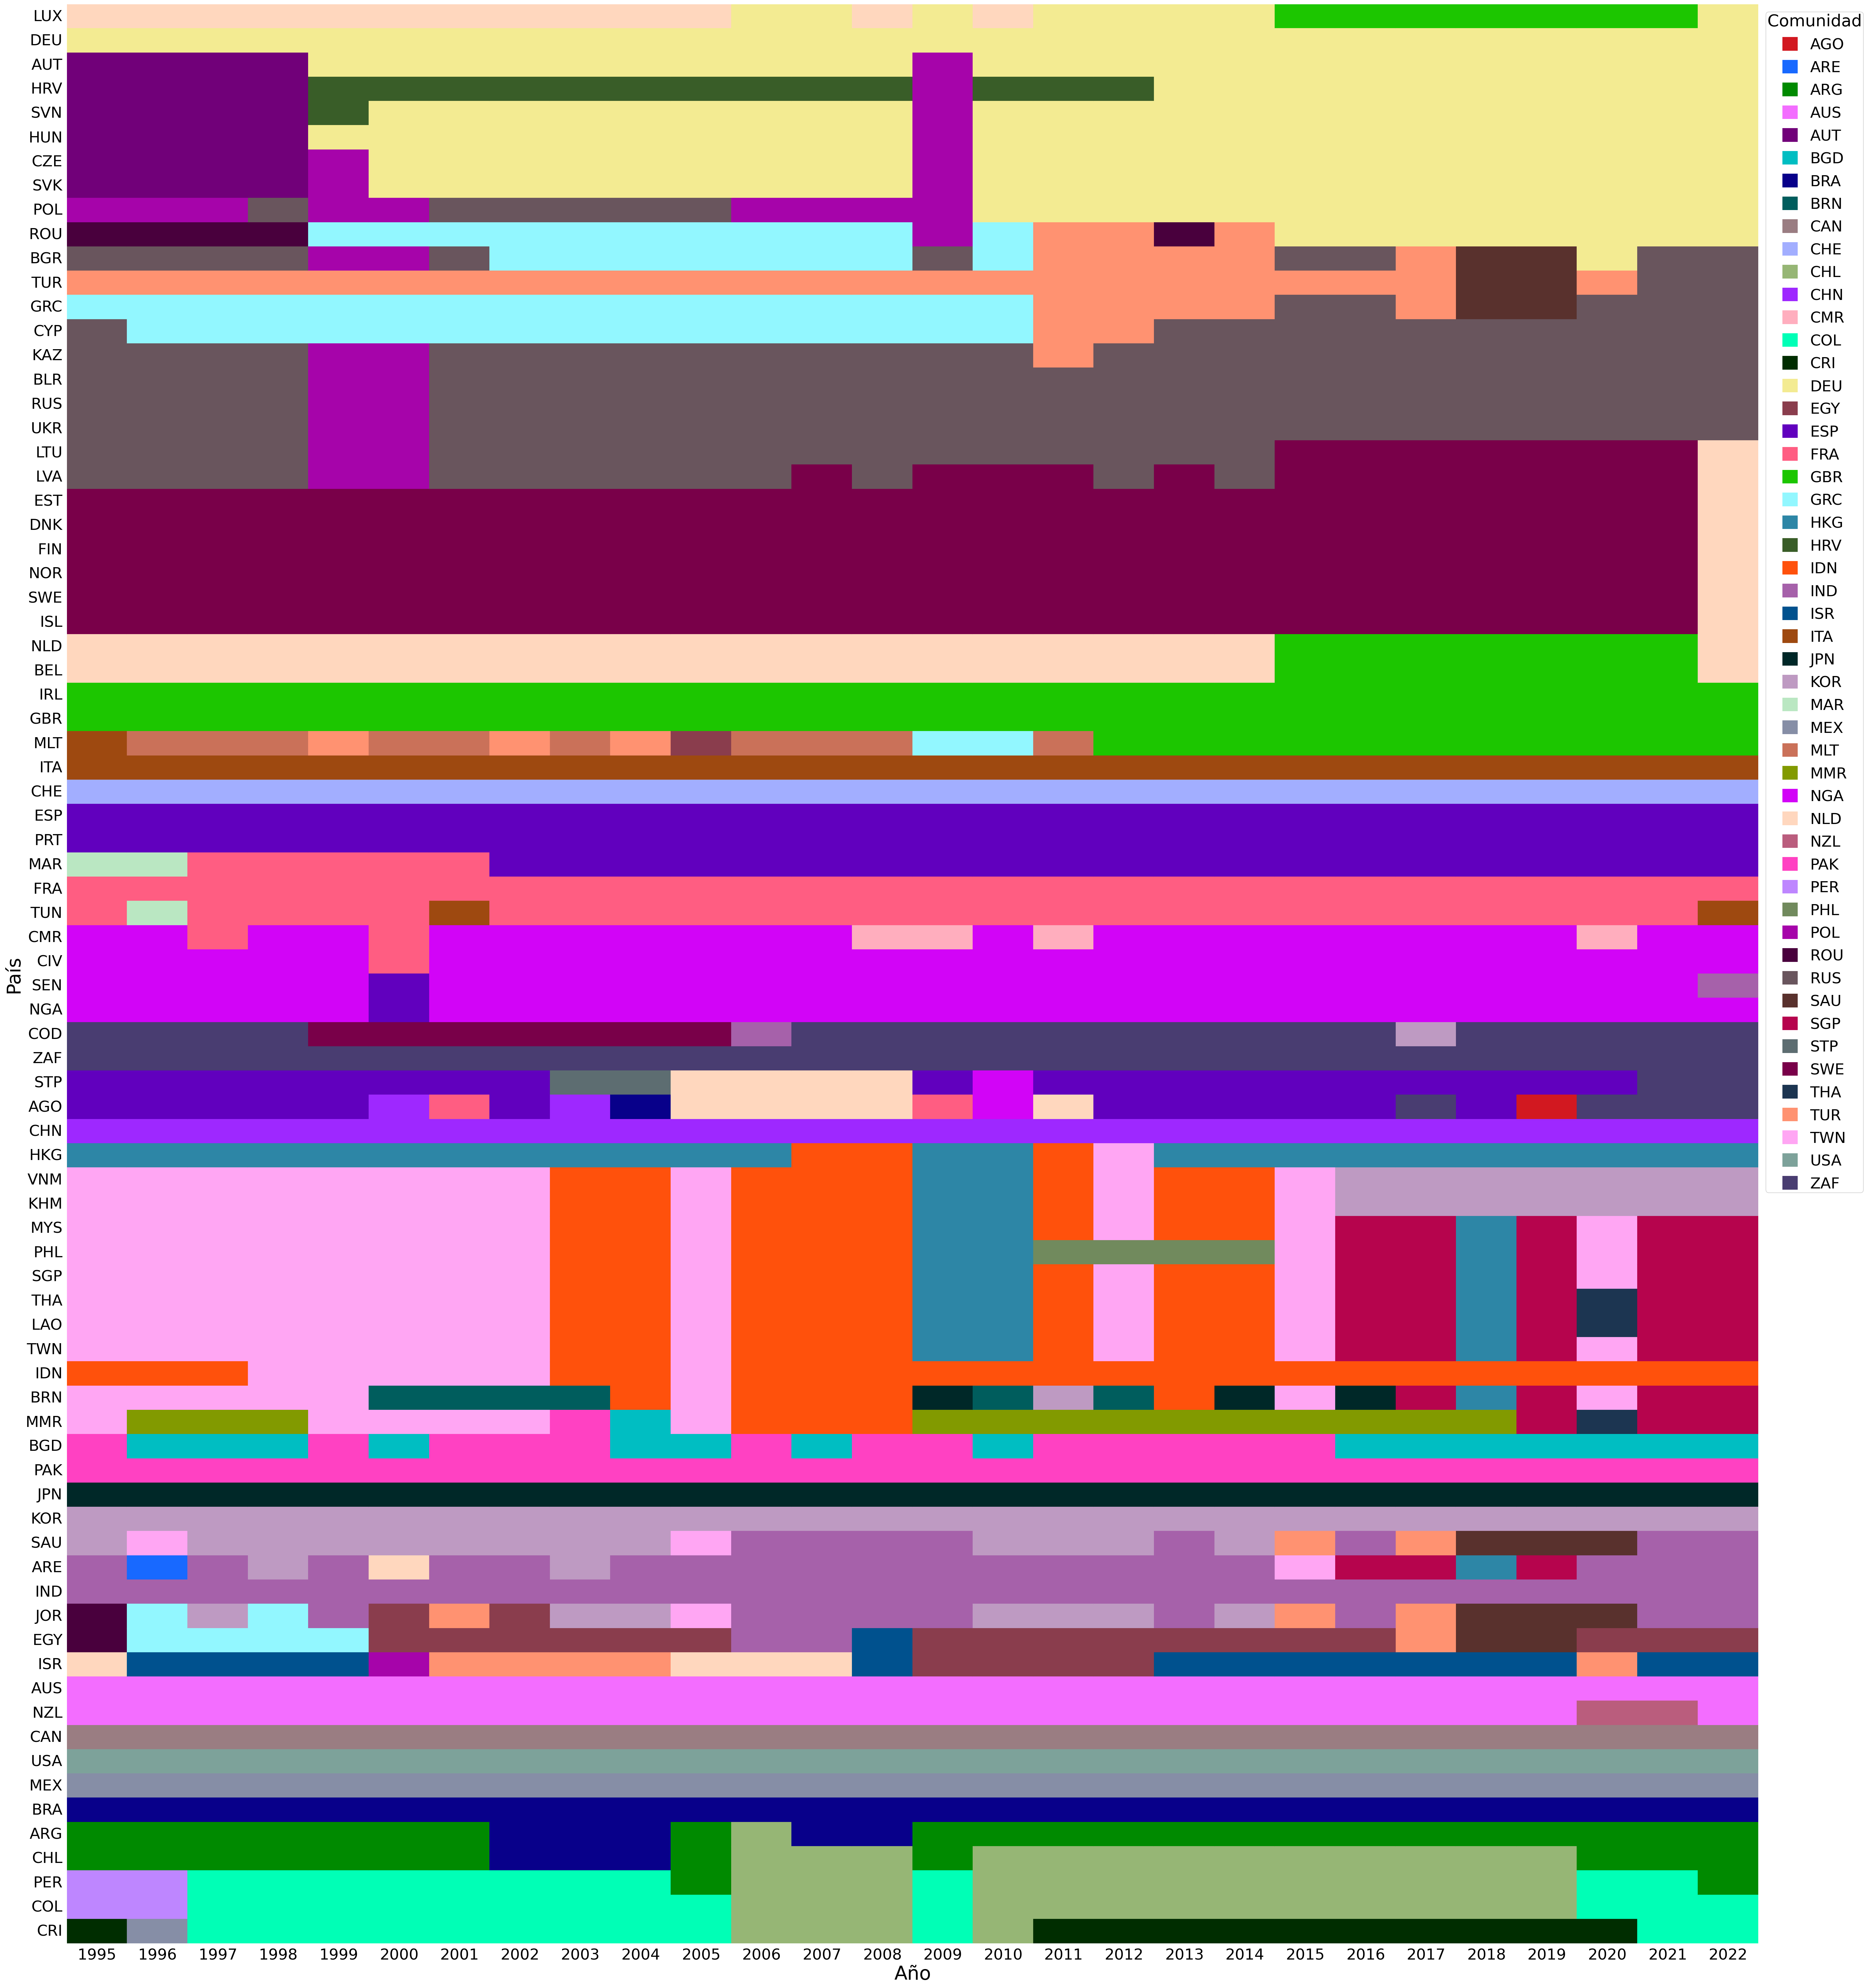
\includegraphics[width=1.1\linewidth]{ComunidadesPorPais.png}
	\caption{\textcolor{blue}{La gráfica muestra a que bloque está integrado la mayoría de la economía de un país. Esto es a que bloque pertenece el 50\%+1 de los sectores de un país. Puede verse cuando dos bloques se unifican. Por ejemplo a partir de 2000, los paies de Europa central y alemania forman un bloque. También se ve cuando un país deja de estar dentro de un bloque por ejemplo, Lituania, letonia y polonia dejan de estar en el bloque de rusia a partir de 2015.}}
\end{figure}

% Calcular modularidad de dividir la economía en bloques de sectores. A ( agropecuario), B(extraccion minera), C(industria), D (electicidad, gas), E 8agua, F Construccion, G (Comercio), H (transporte), I (alojamiento y comida), J (editorial, radifufson telecomunicaciones, tecnología e información), K (financieras), L (inmobiliarias), M (profesionales), N (adm), O, (publica), P (educacion), Q (salud), R (artes), S(otros), T (domesticos.)


\section{Análisis regional}

 %\textcolor{blue}{Analizar la evolución histórica de algunos bloques. En particular, de la Unión Europea, el TLCAN y ASEAN}.







